\section{Mätinstrument}
\textbf{
  HAREC a.\ref{HAREC.a.8.2}\label{myHAREC.a.8.2}
}

\subsection{Presentation av mätvärden}

\begin{wrapfigure}[20]{R}{0.5\textwidth}
  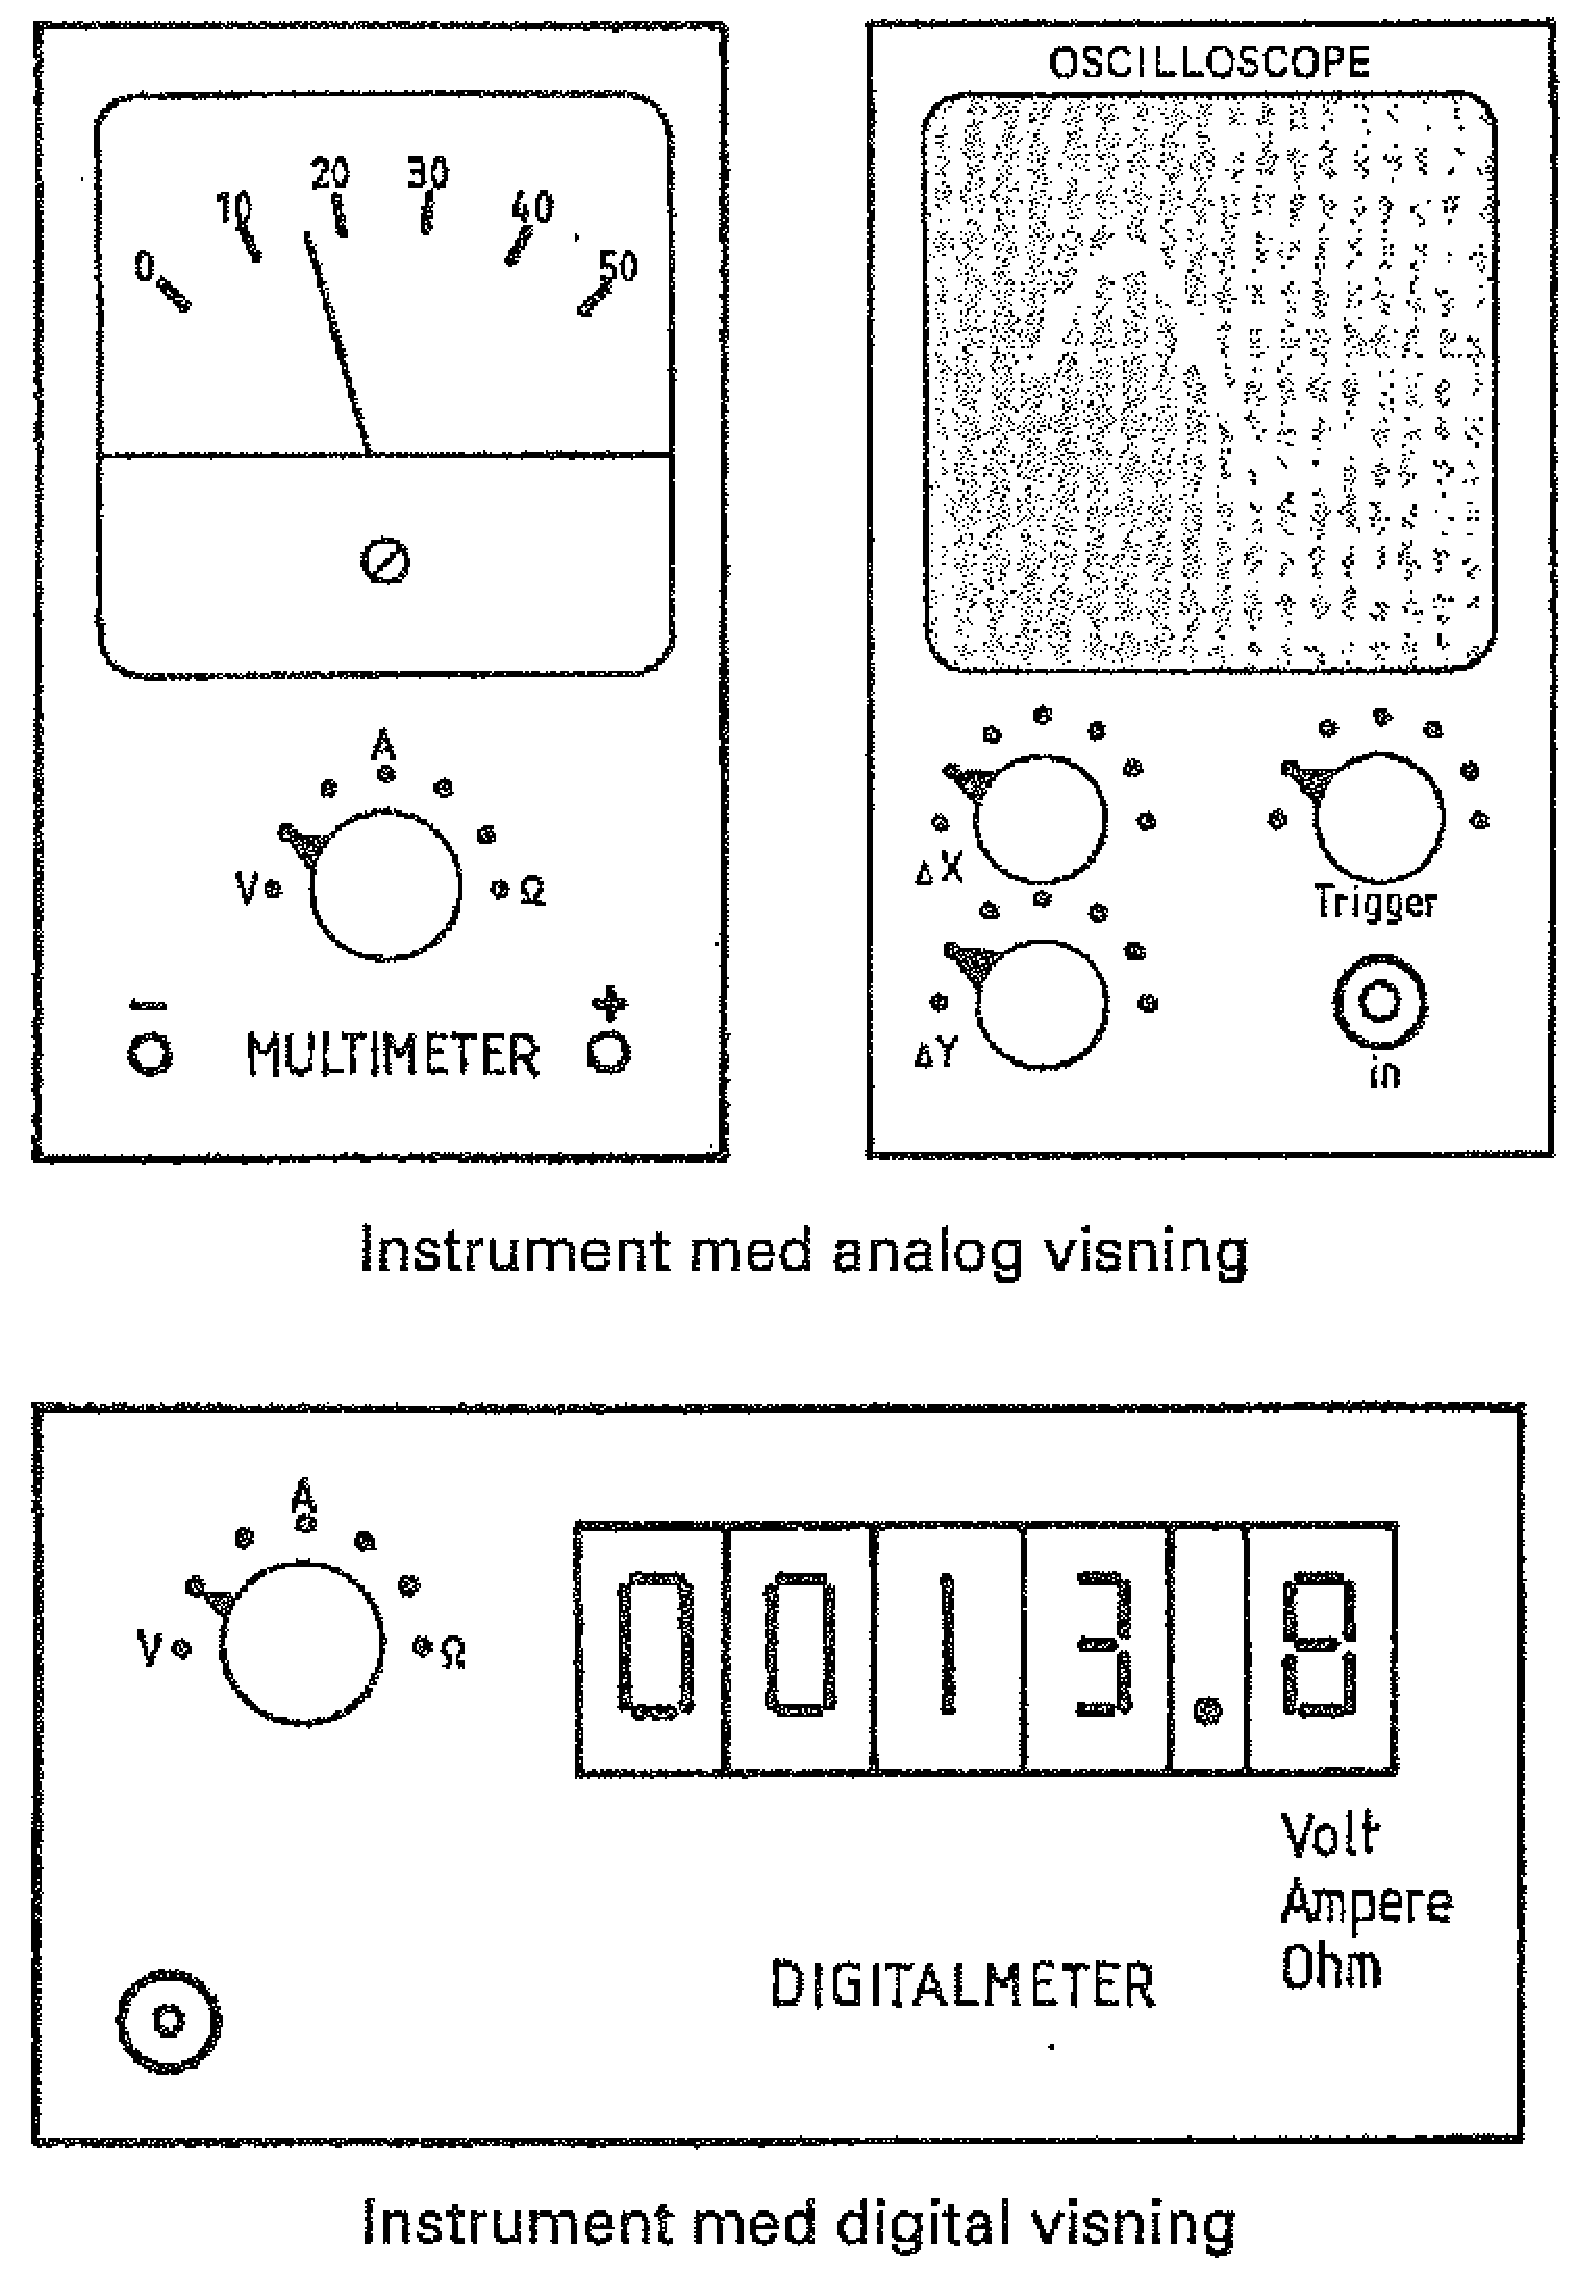
\includegraphics[width=0.5\textwidth]{images/cropped_pdfs/bild_2_8-02.pdf}
  \caption{Presentation av mätvärden}
  \label{fig:bildII8-2}
\end{wrapfigure}

Bild \ref{fig:bildII8-2}

Mätvärden kan presenteras på olika sätt. De vanligaste sätten är
optiska och då med digital eller analog visning. Mätresultat kan även
överföras till dator för vidare bearbetning och visning.

\subsection{Multimeter}
\textbf{
HAREC a.\ref{HAREC.a.8.2.1.1}\label{myHAREC.a.8.2.1.1}
}

Bild \ref{fig:bildII8-2}

Flera mätfunktioner kan utföras med samma basinstrument. Genom
omkoppling mellan olika tillsatser väljer man mätfunktion och
mätområde. Instrumentskalan utformas så att olika slags mätvärden kan
avläsas.  Kombinationer med elektroniska förstärkare och digital
visning etc. är nu vanligt.

\subsection{Vridspoleinstrument}

\begin{figure}
  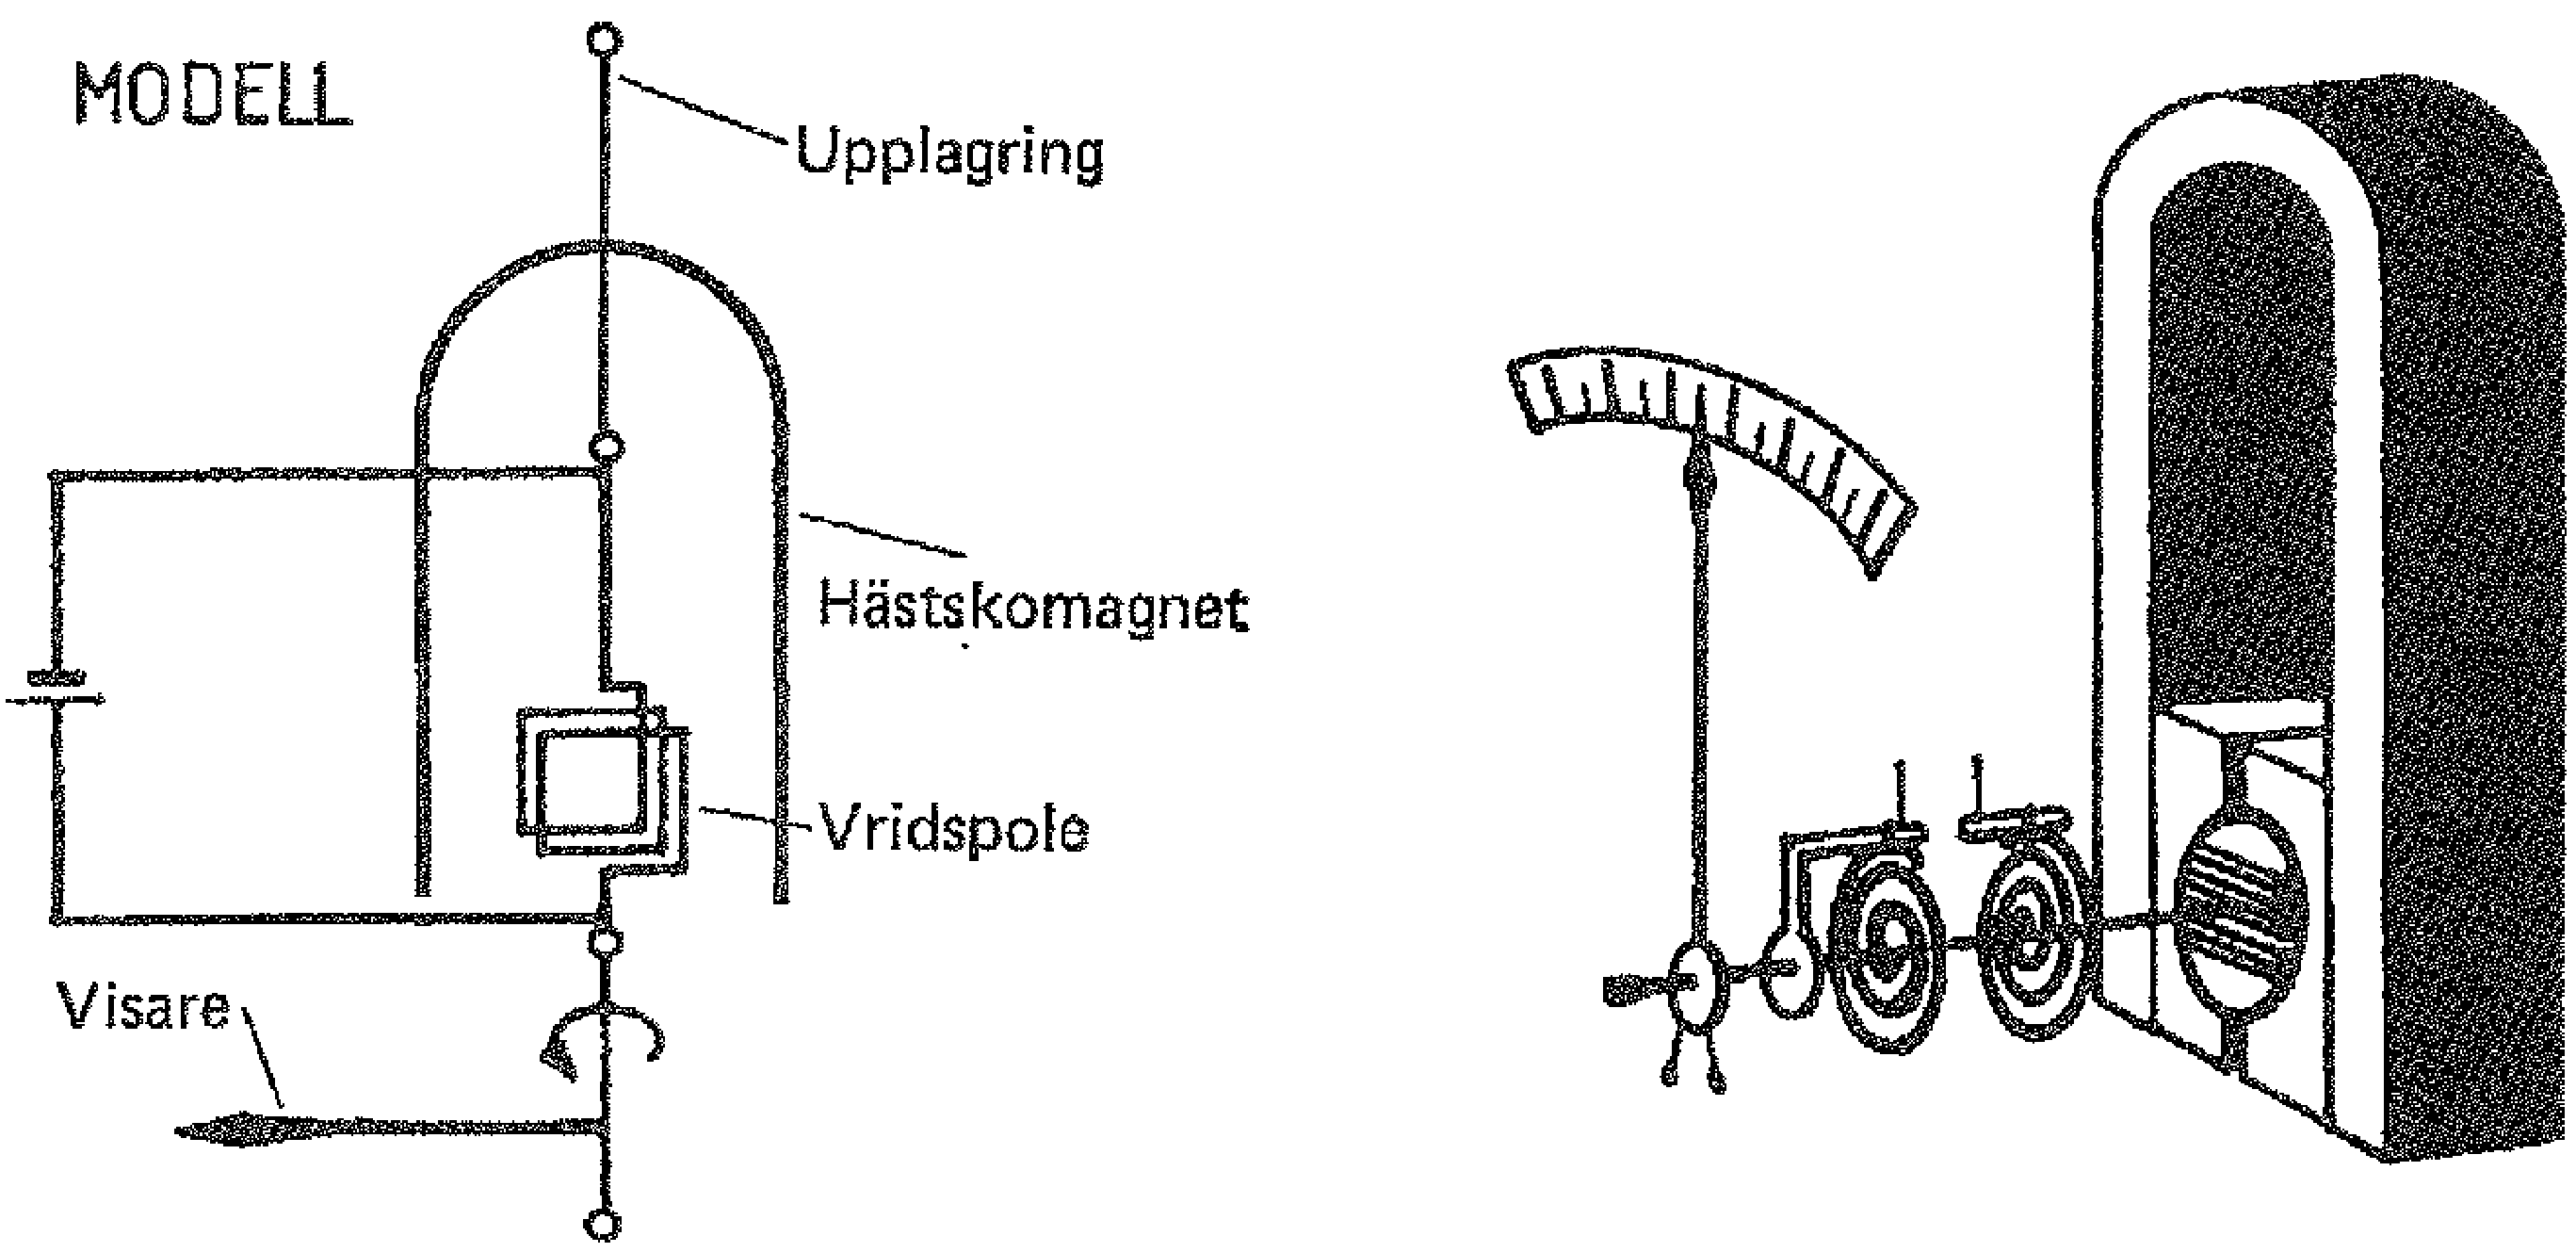
\includegraphics[width=\textwidth]{images/cropped_pdfs/bild_2_8-03.pdf}
  \caption{Vridspoleinstrument}
  \label{fig:bildII8-3}
\end{figure}

Bild \ref{fig:bildII8-3}

Vridspoleinstrument kan bara användas för likströmsmätning, eftersom
visarutslaget beror av strömriktningen.
Instrumentet har låg effektförbrukning och stor noggrannhet.
Visningen är vanligen linjär, men kan göras annorlunda.

Funktion: En spole är upplagrad i fältet av en hästskomagnet När den
ström, som ska mätas, passerar genom den vridbara spolen så alstras
ett magnetfält även i denna. De två magnetfälten påverkar varandra så
att spolen vrider sig. Spolen förses med en visare och en
returfjäder. Ju större ström det flyter genom spolen desto större blir
visarutslaget

\begin{wrapfigure}{R}{0.5\textwidth}
  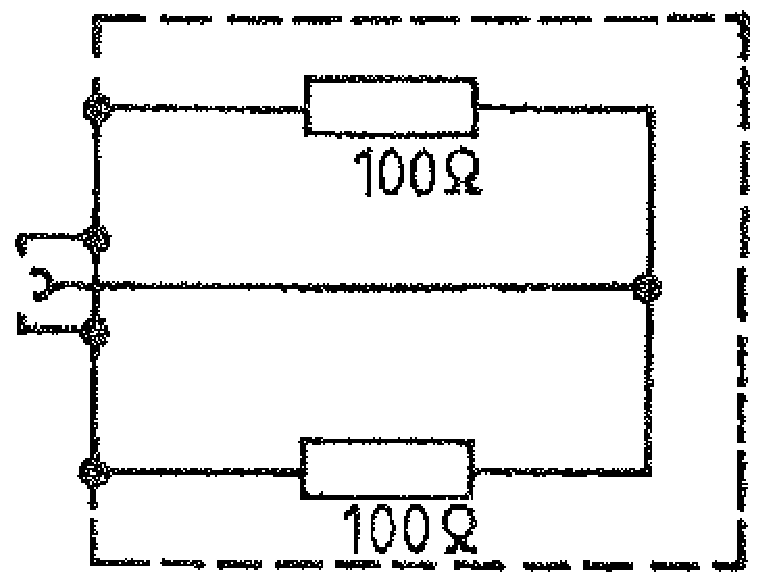
\includegraphics[width=0.5\textwidth]{images/cropped_pdfs/bild_2_8-05.pdf}
  \caption{Konstlast}
  \label{fig:bildII8-5}
\end{wrapfigure}

\subsection{Konstlast}

Bild \ref{fig:bildII8-5}

En konstlast (dummy load) bör ingå i varje amatörradiostation.  Vid
mätning och inställning av t.ex. modulation och uteffekt, är det
lämpligt att belasta sändaren med dess nominella utgångsimpedans.  För
att då undvika att energi strålas ut bör en väl skärmad konstlast
användas.

I moderna amatörradiosändare med koaxialkabel utgång är
utgångsimpedansen 50~Ω.
Konstlasten ska då vara en 50~Ω resistor utan reaktiva egenskaper.
Den kan bestå av en eller flera sammankopplade resistorer.

Sändareffekten ska kunna tas upp utan att resistansen förändras
nämnvärt. Det är viktigt att resistorerna kyls effektivt med luft
eller vätska i ett kärl med tillräckligt utrymme, även när vätskan
expanderar av värmen.  Vätskan får inte vara lättantändlig eller
miljöfarlig.  T.ex. är oljor med PCB förbjudna!

\subsection{Fältstyrkemätare}

\begin{figure}
  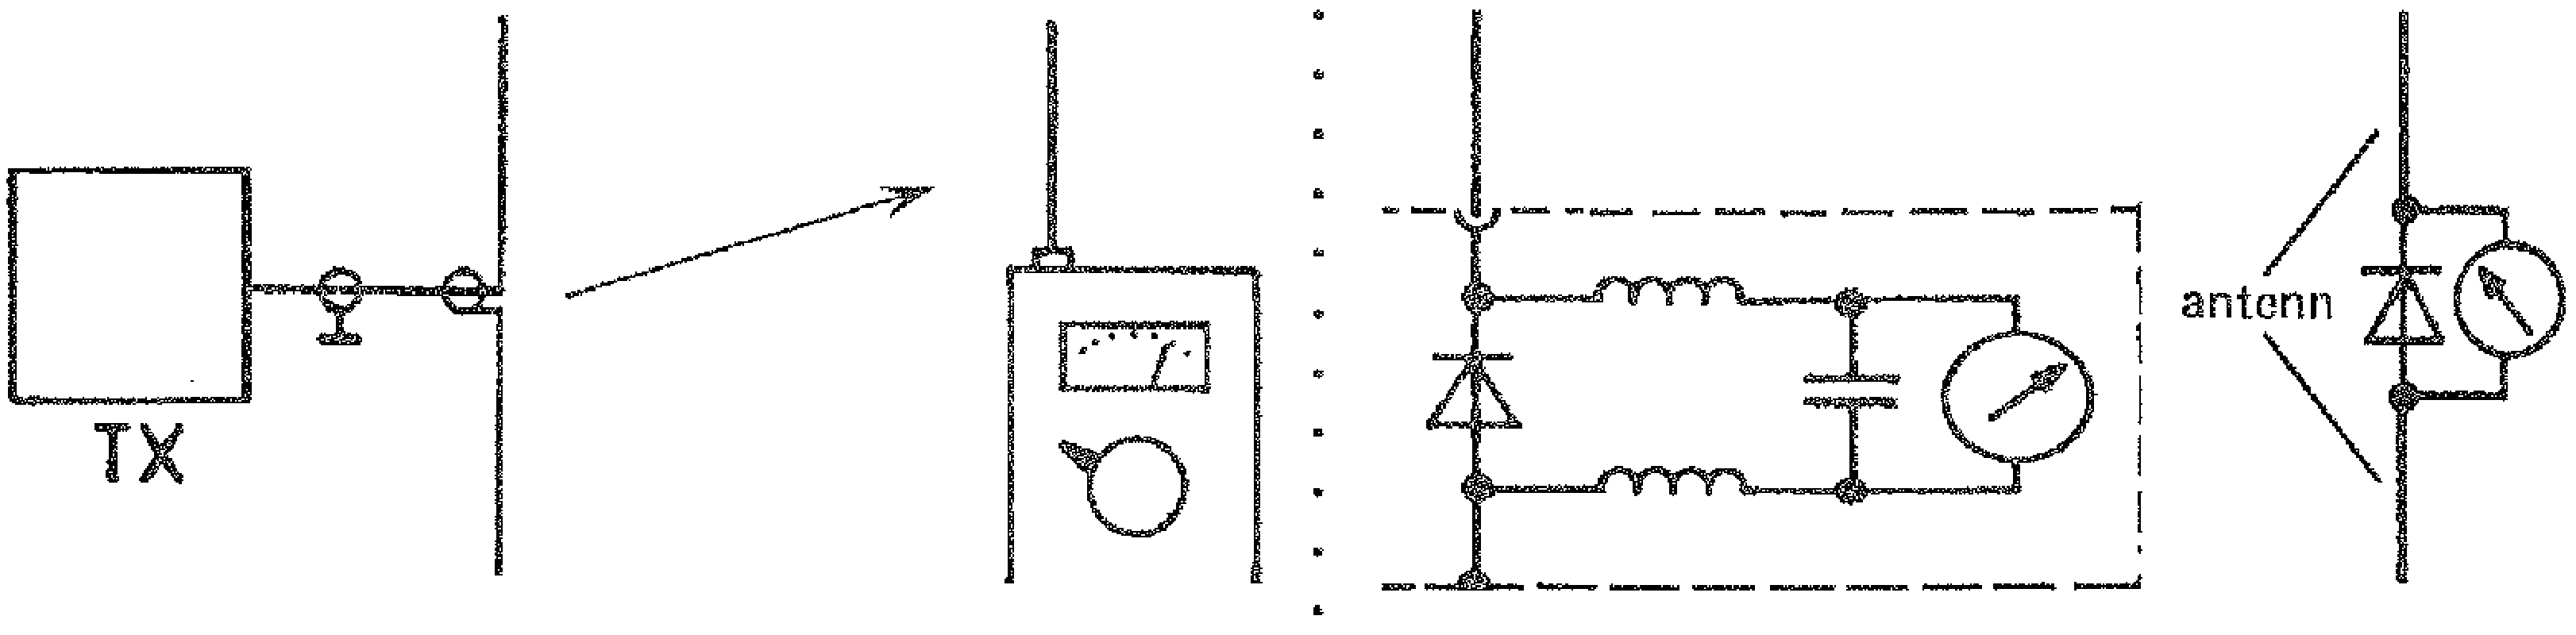
\includegraphics[width=\textwidth]{images/cropped_pdfs/bild_2_8-06.pdf}
  \caption{Fältstyrkemätare}
  \label{fig:bildII8-6}
\end{figure}

Bild \ref{fig:bildII8-6}

Styrkan av elektromagnetiska fält kan bestämmas med fältstyrkemätare.

En fältstyrkemätare är en högfrekvensdetektor, vars utspänning visas
med ett instrument med skala.  Den selektiva kretsen kan bestå enbart
av den avstämda antennen, men även av ytterligare selektiva
kretsar. Instrumentet visar endast relativa värden och används
t.ex. för att bestämma strålningsegenskaperna i sändarantenner och för
antennjustering.  Mätresultatet påverkas även av utstrålning från
andra sändare inom mätarens bandbredd.  Bilden visar en sändare och en
fältstyrkemätare.  Dessutom två enkla fältstyrkemätare.

\subsection{Kalibreringsoscillator}
\textbf{
HAREC a.\ref{HAREC.a.8.2.1.4}\label{myHAREC.a.8.2.1.4}
}

\begin{wrapfigure}[12]{R}{0.5\textwidth}
  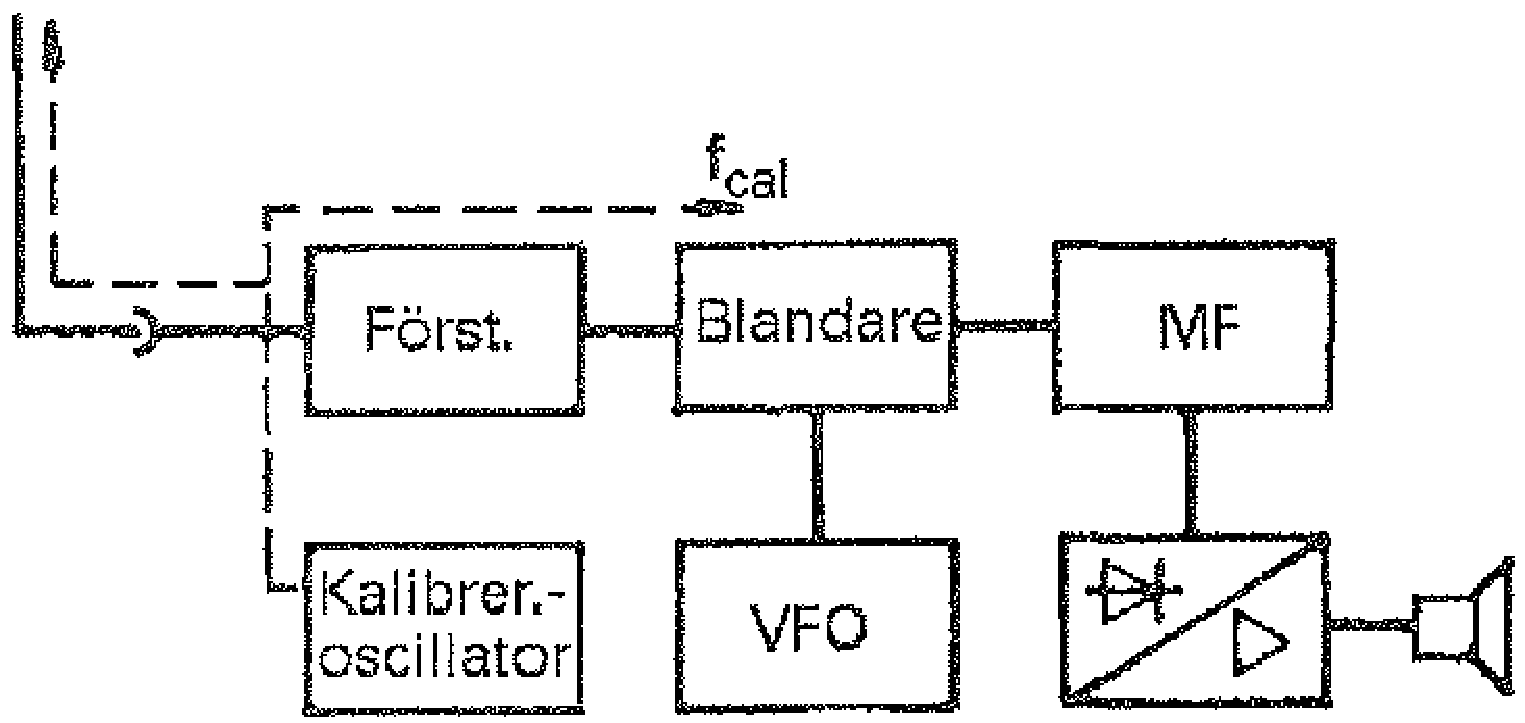
\includegraphics[width=0.5\textwidth]{images/cropped_pdfs/bild_2_8-07.pdf}
  \caption{Kalibreringsoscillator i mottagare}
  \label{fig:bildII8-7}
\end{wrapfigure}

Bild \ref{fig:bildII8-7}

En kalibreringsoscillator används för att frekvenskalibrera andra
apparaters inställningsskalor.  Den är kristallstyrd och avger
särskilt precisa och frekvensstabila signaler.

Oscillatorsignalen förvrängs avsiktligt, så att det utöver
grundfrekvensen även skapas harmoniska övertoner.
En oscillator med t.ex. grundfrekvensen 25~kHz avger på så sätt även
frekvenserna 50~kHz, 75~kHz, 100~kHz, 125~kHz o.s.v.
Man får således en ''kalibreringsfrekvens'' för varje 25~kHz.

Detta övertonsspektrum kan sträcka flera 100~MHz upp. Man
''nollsvävar'' apparat mot närmaste kalibreringsfrekvens och kan
kalibrera t.ex. VFO-skalan.

Användningsområden:
\begin{itemize}
\item Kalibrering av mottagare och
\item Gradering av nya skalor o.s.v.
\end{itemize}

Not: Äldre trafikmottagare har VFO med LC-krets och ofta en inbyggd
kalibreringsoscillator. En kalibreringsoscillator kan i sin tur behöva
kalibreras. Det enklaste sättet är då, att jämföra frekvensen på en
känd rundradiosändare på mellanvåg med kalibreringsoscillatorn.
Dagens mottagare och sändare har syntesoscillator och då behövs
normalt ingen kalibreringsoscillator.

\subsection{Brusmätbrygga}

\begin{wrapfigure}{R}{0.5\textwidth}
  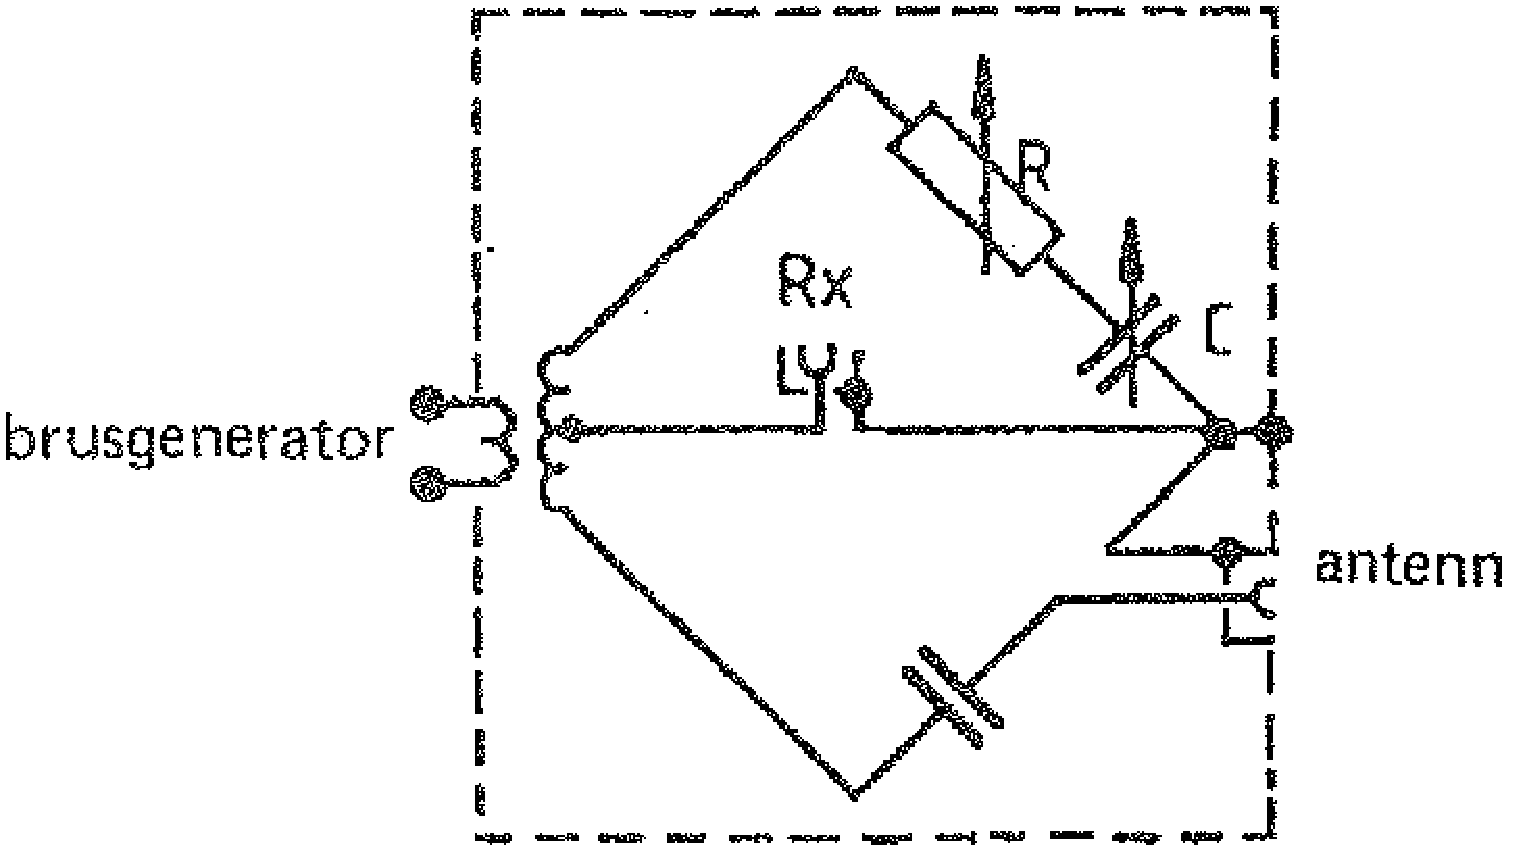
\includegraphics[width=0.5\textwidth]{images/cropped_pdfs/bild_2_8-08.pdf}
  \caption{Brusmätbrygga}
  \label{fig:bildII8-8}
\end{wrapfigure}

Bild \ref{fig:bildII8-8}

Brusmätbryggan används vid mätning i antennsystem. Den består av en
brusgenerator och en Wheatstone-brygga för mätning av resistans och
reaktans.

Till bryggan ansluts en antenn som mätobjekt och en mottagare som
nollindikeringsinstrument för brussignalen. Mottagaren ställs in på
den frekvens där mätvärden önskas. Bruset hörs svagast när bryggan är
injusterad. Man kan då avläsas mätvärdena för \(R\) och \(X\). Mäter
man vid flera frekvenser, kan t.ex. ett impedansdiagram upprättas.

\subsection{Ståendevågmeter (SVF-meter)}
\textbf{
HAREC a.\ref{HAREC.a.8.2.1.3}\label{myHAREC.a.8.2.1.3}
}

\begin{figure}
  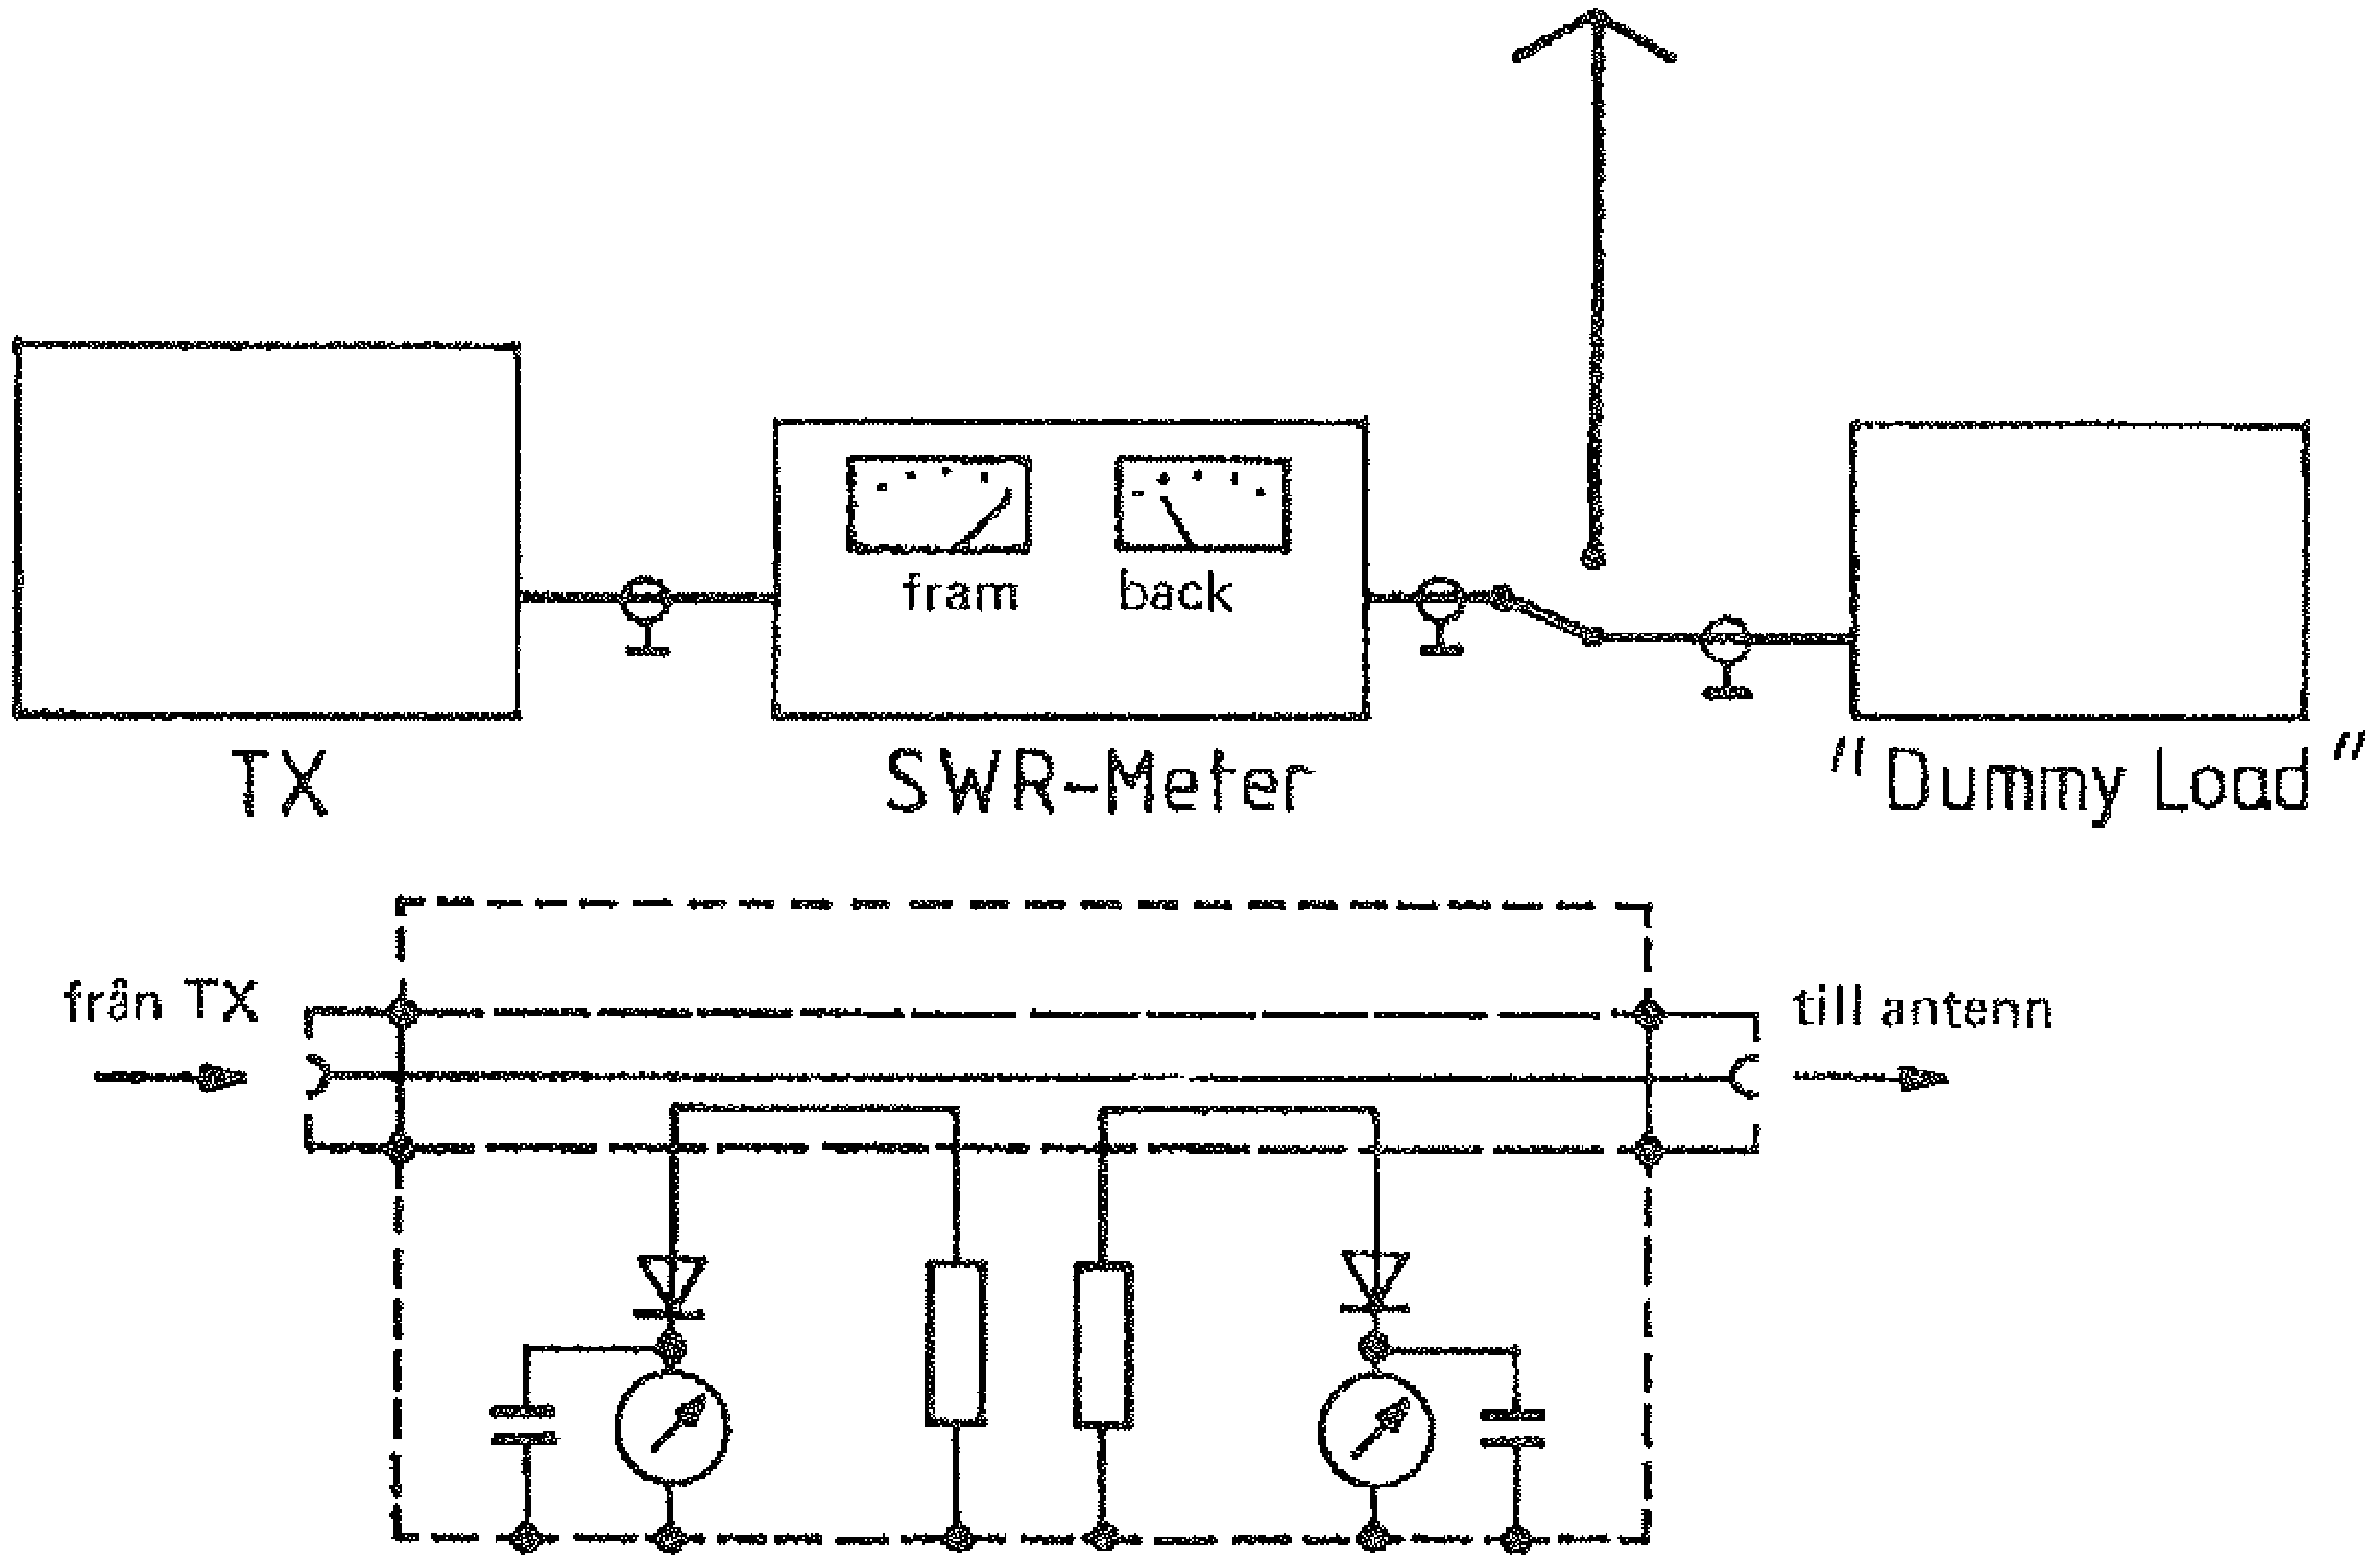
\includegraphics[width=\textwidth]{images/cropped_pdfs/bild_2_8-09.pdf}
  \caption{SVF-meter, princip och inkoppling}
  \label{fig:bildII8-9}
\end{figure}

Bild \ref{fig:bildII8-9}

När en transmissionsledning eller apparat ansluts till en annan med
avvikande impedans, kommer HF-energi att reflekteras i övergången.

Med ståendevåg-förhållande (SVF) eller Standing Wave Ratio (SWR)
menas förhållandet mellan den effekt som flyter framåt respektive
bakåt i en transmissionsledning.

Användningområden för SVF-meter:
\begin{itemize}
\item Mätning av framåtgående effekt.
\item Mätning av bakåtgående effekt.
\item Bestämning av SVF.
\item Bestämning av resulterande, relativ effekt.
\end{itemize}

Anmärkning: Vid bestämning av absolut effekt måste
anslutningsimpedansen vara lika i instrument och transmissionsledning.

SVF-metern är ett av de mest användbara instrumenten vid
HF-mätningar. En SVF-meter kan ha separata instrument för fram-
respektive backeffekt eller ett gemensamt.

SVF-metern kan vara ständigt inkopplad t.ex. mellan sändare och
antenn, men ska då kunna tåla effektutvecklingen. En SVF-meter kan
alstra övertoner, vilka kan medföra störningar. Orsaken är
olinjäriteten halvledardioderna i instrumentet.

\subsection{Frekvensräknare}
\textbf{
HAREC a.\ref{HAREC.a.8.2.1.5}\label{myHAREC.a.8.2.1.5}
}

\begin{wrapfigure}{R}{0.5\textwidth}
  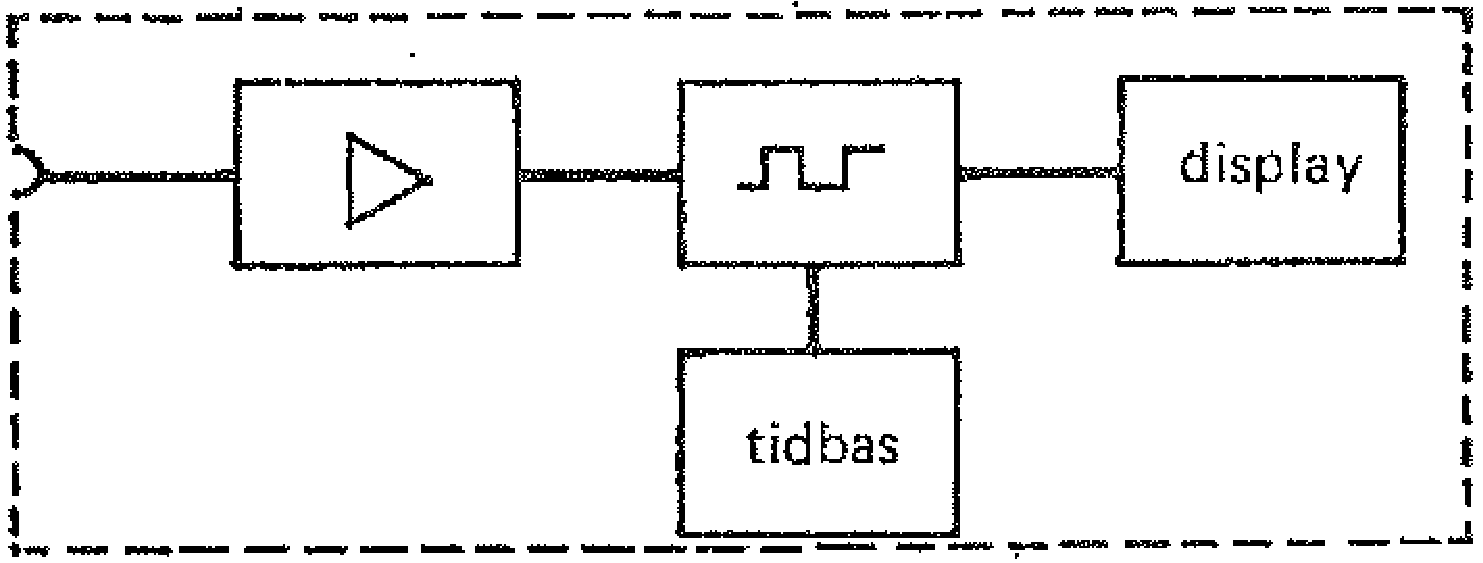
\includegraphics[width=0.5\textwidth]{images/cropped_pdfs/bild_2_8-10.pdf}
  \caption{Frekvensräknare}
  \label{fig:bildII8-10}
\end{wrapfigure}

Bild \ref{fig:bildII8-10}

Frekvensräknaren, som är ett digitalt instrument, används för att
bestämma oscillatorfrekvensen i sändare, mottagare m.m.

I frekvensräknaren räknas antalet svängningar i den aktuella
inkommande signalen under en bestämd tidsenhet. Först förstärks
signalen i en analog förstärkare och omvandlas till kantvågspulser. En
elektronisk ''kontakt'', en s.k. gate, släpper därefter den behandlade
ingångssignalen vidare till en digital räknare under en viss
tid. Detta sker med stor precision och i ett periodiskt
förlopp. Antalet pulser räknas under genomsläppsperioden. Resultatet
motsvarar insignalens frekvens.

Resultatet visas som siffror i ett fönster. Noggrannheten i den
s.k. tidbasen erhålls med en kristallstyrd oscillator, vars frekvens
delas ner till önskat värde.

\subsection{Dip-meter}

\begin{wrapfigure}{R}{0.5\textwidth}
  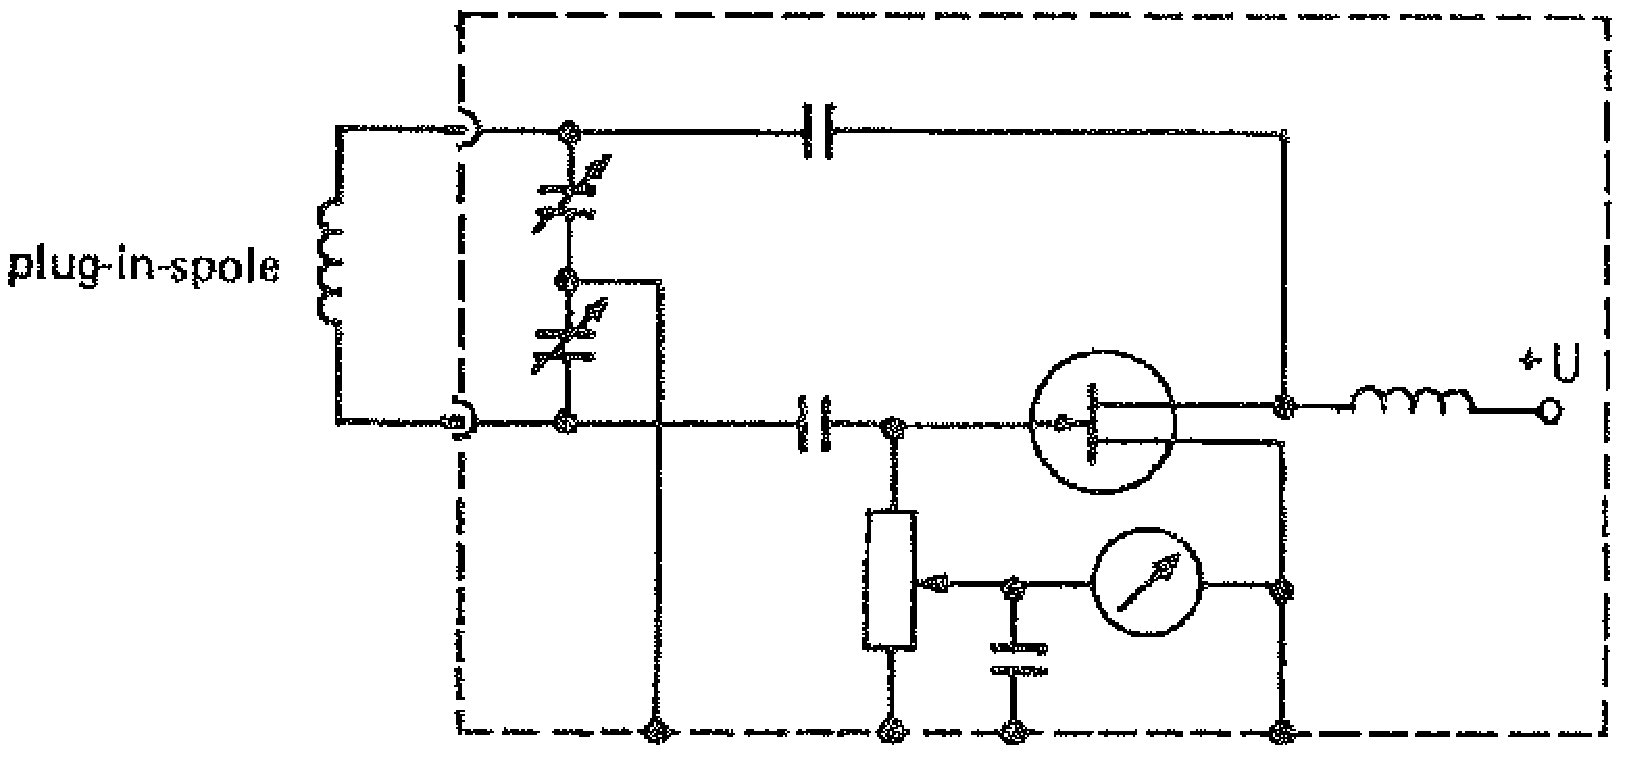
\includegraphics[width=0.5\textwidth]{images/cropped_pdfs/bild_2_8-12.pdf}
  \caption{Dip-meter}
  \label{fig:bildII8-12}
%\end{wrapfigure}

%\begin{wrapfigure}{R}{0.5\textwidth}
  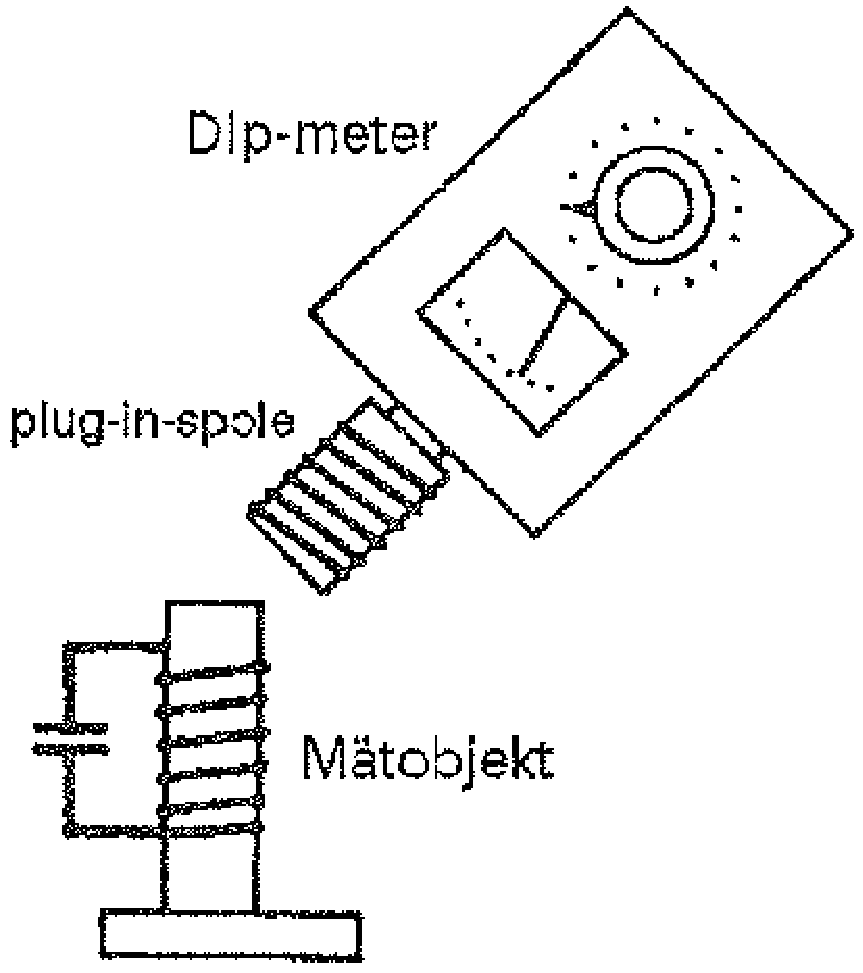
\includegraphics[width=0.5\textwidth]{images/cropped_pdfs/bild_2_8-13.pdf}
  \caption{Mätning med dip-meter}
  \label{fig:bildII8-13}
\end{wrapfigure}

Se bild \ref{fig:bildII8-12} och \ref{fig:bildII8-13}.

Dip-metern är i princip en oscillator med variabel frekvens och
utbytbara induktorer för olika frekvensområden.
Den används för att bestämma resonansfrekvensen på passiva och aktiva
svängningskretsar samt vid bestämning av induktanser och kapacitanser.

Noggrannheten är ca 3~\%.

Funktion: Instrumentet avger alternativt reagerar för en HF-signal med
viss frekvens. Resonansfrekvensen i dip-meterns svängningskrets är
steglöst variabel och frekvensvärdet kan avläsas på en skala.

Vid mätning av resonansfrekvensen i en passiv svängningskrets kopplas
dip-meterns induktor induktivt till kretsen. När resonansfrekvensen i
kretsen och dip-metern överensstämmer, ändras belastningen i
dip-meterns svängningskrets varvid instrumentet uppvisar en
strömminskning -- en ''dip''. Frekvensen avläses då på skalskivan.

Vid mätning på en aktiv svängningskrets, d.v.s. som drivs av någon
HF-källa, uppstår i stället en strömökning vid resonans vilket också
visas på instrumentet.

Induktansen i en svängningskrets kan bestämmas med dip-metern, om
kapacitansen är bekant. På motsvarande sätt kan en obekant kapacitans
bestämmas om induktansen i svängningskretsen är bekant.

Namnet grid-dipmeter kommer från elektronrörsepoken. Ändringar i
gallerströmmen (grid current) i ett oscillatorkopplat elektronrör
används som indikation på att en svängningskrets är i resonans. Då
minskar gallerströmmen -- det blir en ''ström-dip''. Numera används en
transistor i stället för röret och instrumentet benämns dip-meter.

\subsection{Oscilloskop}
\textbf{
HAREC a.\ref{HAREC.a.8.2.1.6}\label{myHAREC.a.8.2.1.6}
}

\begin{figure}
  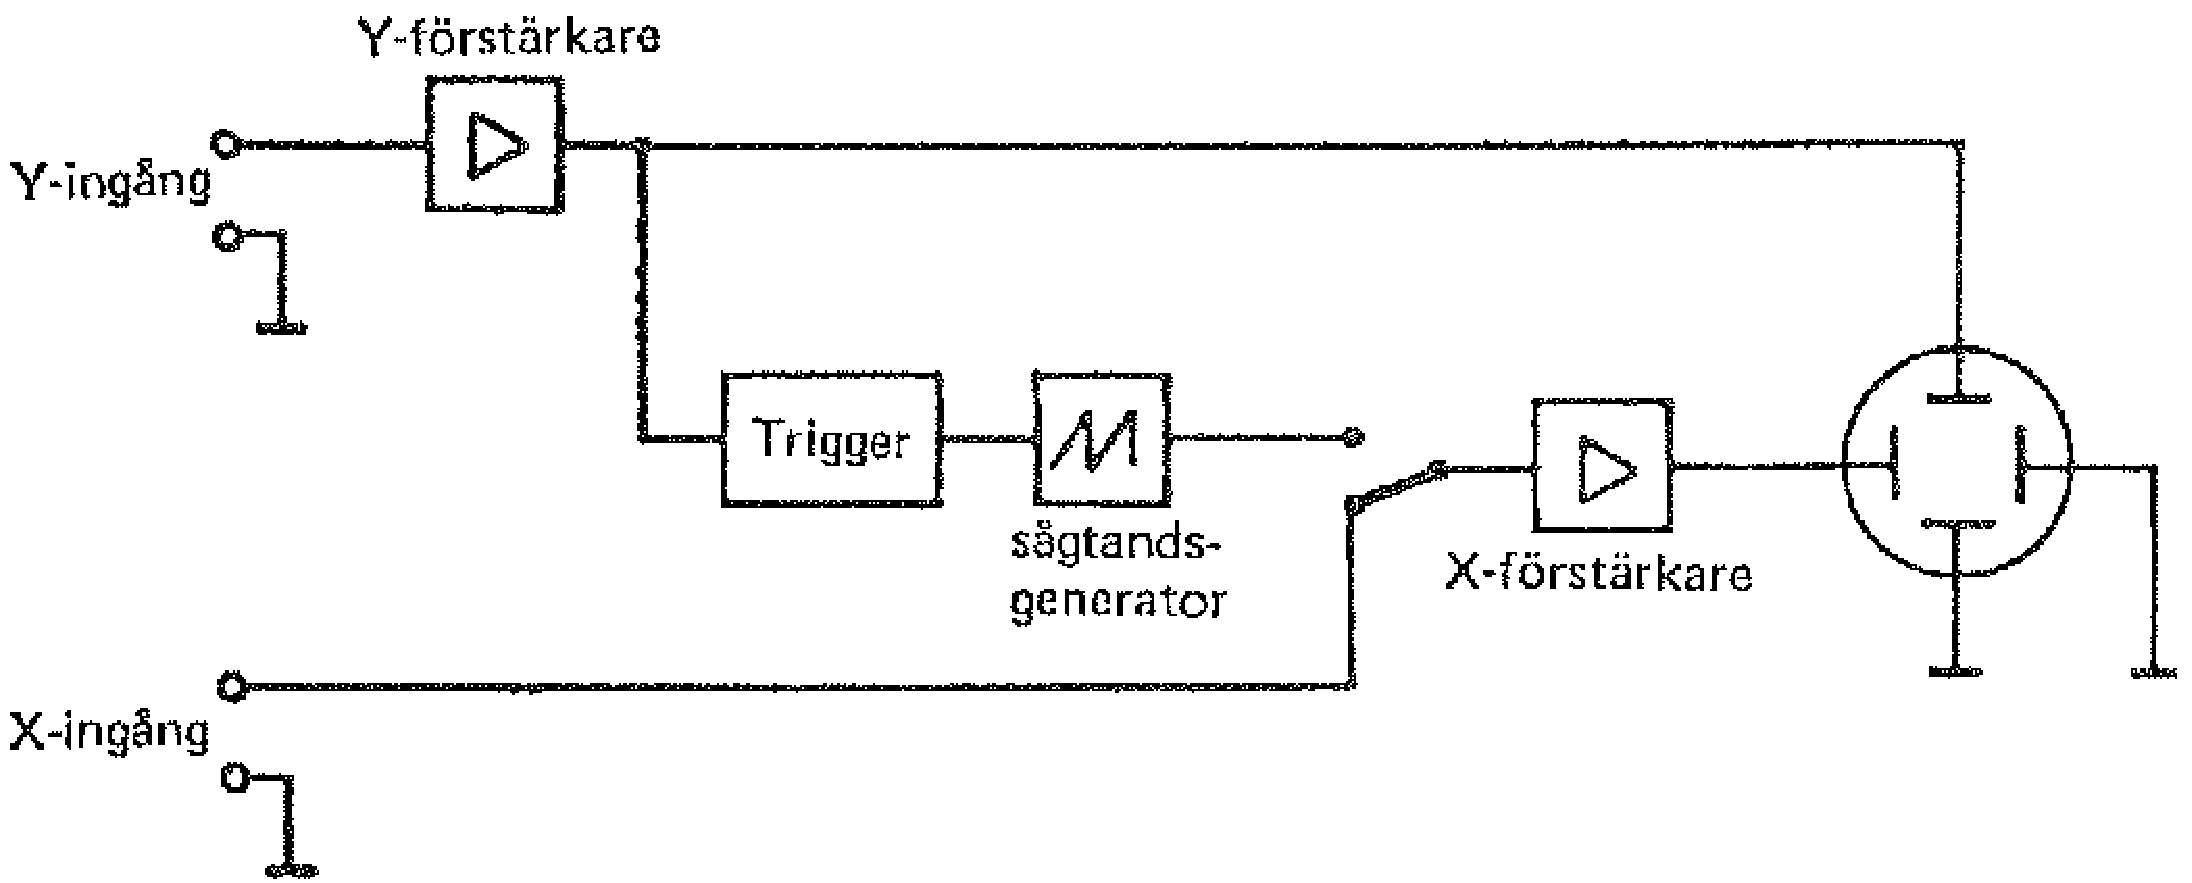
\includegraphics[width=\textwidth]{images/cropped_pdfs/bild_2_8-14.pdf}
  \caption{Oscilloskop}
  \label{fig:bildII8-14}
\end{figure}

Bild \ref{fig:bildII8-14}

Oscilloskopet är ett mycket användbart instrument. Mycket snabba
förlopp kan med fördel studeras på en oscilloskopskärm.

Spänningsförlopp kan visas som funktion av tiden. Tillsammans med
andra instrument kan frekvenskaraktäristiken i filter,
modulationskvalitet o.s.v. åskådliggöras.

Oscilloskopet består av ett katodstrålerör, där styrningen av
katodstrålen sker med hjälp av X- och Y-förstärkare och en s.k.
triggerförstärkare. Den signal som ska mätas ansluts vanligen till
Y-förstärkaren medan en tidbasgenerator som alstrar en sågtandformad
signal ansluts till X-förstärkaren.  Bilden visar ett blockschema på
oscilloskop.

Moderna oscilloskop digitaliserar signalen efter ingångsförstärkaren,
och läggs sedan i minne, där den sågtandsformade signalen är ersatt med en
räknare som placerar det i minnet. Sen presenteras bilden på bildskärmen
eller på en ansluten dator.

Gemensamt för analoga och digitala oscilloskop är i stort samma handhavande.

Man ansluter en eller flera signaler till ingångarna, justerar ingångssteget
så att hela vågformen fångas och att det är god amplitud, så den syns men inte
klipps.
Ibland väljer man att göra vågformerna mindre, för att man ska kunna
arrangera dem på ett bra sätt på skärmen.
Ibland väljer man att klippa vågen för att man enbart vill se tiden för en
kant tydligt.

En viktig sak är att sätta en bra trigg-punkt, så att man får en tydlig bild.
Ett vanligt misstag är att sätta triggpunkten på en plats på vågen där den är
väldigt flack eller så att den kan trigga på flera olika ställen på vågformen,
det gör att efterföljande bilder triggar och får suddiga eller dubbla bilder,
då brukar man justera trigg-punkten så att man får en tydlig bild.

Man justerar också tidbasen för att ha rätt skala på tidsaxeln, så man ser en
eller ett fåtal cyckler, eller ibland över längre tid för att se variationer.
Man kan också fördröja svepet för att kunna se en viss del efter trigg-punkten.

Oscilloskop har nu mer ofta inbyggda mätfunktioner.
Det är behändigt att snabbt få en uppfattning om periodtider, frekvenser,
amplituder mm. men dessvärre är mätprecissionen ofta kraftigt lidande, och
det ska inte övertolkas.
T.ex. är frekvensmätningen inte bättre än hur bra placeringen av markörerna är,
så det är sällan tillförlitligt bättre än 2 siffrors noggrannhet.

Rätt använt är oscilloskop dock ett fantastiskt mätinstrument.

\subsection{Spektrumanalysator}
\textbf{
HAREC a.\ref{HAREC.a.8.2.1.7}\label{myHAREC.a.8.2.1.7}
}

En spektrum-analysator visar amplituden för olika frekvenser över ett visst
frekvensområde.
Detta är som kontrast till oscilloskopet som visar amplitud för en signal
över tiden.

En spektrumanalysator kan styras för att svepa över olika frekvensområden.
Oftast när man startar den så sveper den från lägsta till högsta frekvens.
Det kan vara behändigt för att få en första översikt.
För en specifik mätning ställer man in start och stop frekvens, eller
alternativt en center-frekvens och ett span.

För att kunna göra bättre avläsningar kan man sätta markörer, så att man kan
avläsa frekvens och amplitud för den punkten.
Ibland sätter man dubbla frekvensen för att avläsa skillnaden i amplitud,
vilket kan vara relevant för filter eller avläsa den relativa styrkan på ett
sidband.

En spektrum-analysator består förenklat av en svep-bar oscillator,
variabelt filter på mellan frekvensen, en detektor och ett ställbart
filter från detektorn.

Den variabla oscillatorn sveper så att det tänkta frekvensområdet täcks,
ofta med ett bestämt antal punkter, t.ex. 801, där varje punkt är mätning på
en specifik frekvens.
Ibland kan man anpassa antalet punkter för att få mätningen gå snabbare,
mot att man får en lägre upplösning.

Filtret sätter bandbredden på mätningen, och det kan gå i 1--3 steg, t.ex.
3~Hz, 10~Hz, 30~Hz, osv. till 3~MHz.
För vissa specifika mätändamål, som t.ex. för EMC mätningar, behöver man ha
filter av rätt bandbredd och dessa är extra optioner.

Detektorn kan vara topp-detektor eller RMS detektor, det kan finnas flera.
För specifika mätändamål som t.ex. EMC mätningar behöver man specifik detektor.

Efter detektorn finns ett filter, ofta benämnt med video-bandbredd, som
medelvärdesbildar detektorns ampltitudestimat över tiden.
Oftast regleras det automatiskt med bandbredden på filtret, eftersom smalare
filter behöver proportionerligt längre tid för att ge ett bra resultat.
Sveptiden beror därför på antalet punkter för frekvenser, bandbredd på filtret
och video-bandbredden.
Ibland kan man styra video-bandbredden manuellt för att få en längre tid, då
det kan vara gynnsamt för att få en tydligare bild, dvs. ta bort brus och
störningar som enbart skapar variationer för att man inte observerar ett bra
medelvärde.

\subsection{Nätverksanalysator}

En nätverksanalysator (eng. network analyser) används för att mäta hur mycket
signal som går igenom en koppling, t.ex. filter eller förstärkare, eller hur
mycket signal som reflekteras tillbaka från t.ex. en antenn.
Ibland kallas detta även för antenn-analysator.

En nätverksanalysator som enbart kan mäta amplituder kallas ibland för
skalär nätverksanalysator (eng. Scalar Network Analyzer -- SNA).
En spektrumanalysator med en så kallad tracking generator, som genererar en
signal med samma frekvens som man analyserar, kan agera SNA.

En nätverksanalysator som mäter fasen både på utgående och inkommande signal
kan även mäta fasförskjutningen, och då kan man representera fasen både som
komplex storhet eller med polära koordinater, dvs. amplitud och fas.
En sådan nätverksanalysator kallas för vektornätverksanalysator (eng.
Vector Network Analyzer -- VNA).

Användningsmässigt liknar en nätverksanalysator en spektrum-analysator, men
med flera väsentliga skillnader.
För att få korrekt mätning av amplitud och fas läggs större vikt vid att göra
kalibrering, något som görs för att kompensera varierande amplitud och fas
för olika frekvenser.
Vid kalibrering använder man ofta last (eng. load), kortslutning (eng. short)
samt öppen port (eng. open) mätning av kalibreringsreferenser.
För två-ports mätning använder man även en genomföring (eng. through) för att
få port-till-port egenskaperna korrekt.
Efter kalibrering av instrumentet så korrigeras mätningarna, och ibland kan
skillnaderna vara drastiska.

Nätverksanalysatorn har därtill ofta ett stort antal olika sätt att presentera
mätresultaten så att man kan mäta enligt scatter-modellen, return loss (RL),
VSWR, Schmitt-diagram och så vidare.
Det gör att en nätverksanalysator kan vara ett kraftfullt verktyg som korrekt
använt kan ge god insikt i hur en krets beter sig.
